%% OptiVision --- research paper built from the completed Q1--Q10 investigation
%% (branch research-investigation; primary source reports/research/PAPER_SUMMARY.md).
%% This file is independent of optivision.tex, which records an earlier thesis.
%% Build: tectonic -X compile optivision_research.tex   (from this directory)
%% Figures: python paper/make_figs_research.py           (from the repo root)
\documentclass[conference]{IEEEtran}
\IEEEoverridecommandlockouts

\usepackage{cite}
\usepackage{amsmath,amssymb}
\usepackage{graphicx}
\graphicspath{{figs/}{./}}
\usepackage{booktabs}
\usepackage{multirow}
\usepackage{url}
\usepackage[hidelinks]{hyperref}

\newcommand{\ms}{\,ms}

\begin{document}

\title{Quality-Constrained Compression of Multi-Vector Retrievers:\\
Compression Axes, Certification Difficulty,\\
and the Boundaries of What Generalizes}

%% TODO before submission: confirm author list, affiliations and e-mail addresses.
\author{
\IEEEauthorblockN{T Rithik Krishna\IEEEauthorrefmark{1},
Amgovath Navanitha\IEEEauthorrefmark{1},
Badavath Akhila\IEEEauthorrefmark{1},
E. Sathiya Lakshmi\IEEEauthorrefmark{2}}
\IEEEauthorblockA{\textit{Department of Emerging Technologies},
\textit{Mahatma Gandhi Institute of Technology (Autonomous)}\\
Affiliated to Jawaharlal Nehru Technological University Hyderabad,
Gandipet, Hyderabad 500075, Telangana, India\\
\IEEEauthorrefmark{1}\{23261a6753, 23261a6704, 23261a6709\}@mgit.ac.in \quad
\IEEEauthorrefmark{2}sathiyalakshmi\_et@mgit.ac.in}
}

\maketitle

\begin{abstract}
Multi-vector late-interaction retrievers store hundreds of vectors per page, which makes
their indexes large. We study post-hoc, training-free compression of fixed page
embeddings along three axes: vector count (Ward merging with per-page budgets), dimension
(PCA) and quantization (int8, centred int4, binary). We evaluate four visual encoders
(ColPali~v1.3, ColQwen2~v1.0, ColQwen2.5~v0.2 and the 2,560-dimensional ColEmbed~4B) on
ViDoRe~V1 DocVQA and InfoVQA, plus a text ColBERT on SciFact, with pre-registered
hypotheses. Within this tested set, fewer stored vectors is the only axis that reduces
exhaustive search cost, which we measured to be linear in stored vectors over the tested
range. Merging to a quarter of the vectors keeps nDCG@5 within 1.1 points of float32 on
every 128-dimensional dataset measured, and merging beats random pruning. Per-vector int8
and centred int4 are near-lossless on every encoder measured, whereas dimension reduction
is model-dependent: harmful at 128 dimensions, nearly free to one eighth of the width at
2,560. The axes interact: compression factors do not multiply, and PCA followed by coarse
codecs is consistently antagonistic. DocVQA admits far less certified compression than
InfoVQA mainly because its quality is harder to certify, not because it is less
compressible. To select a configuration with a statistical statement, we apply known
fixed-sequence testing with exact betting p-values. This bounds the probability of
deploying a configuration below target by $\delta$ under i.i.d.\ queries and a fixed
corpus, and the bound held in 27 of 27 frozen held-back cells. No distribution-free
method can certify a 0.99 retention target with 225 or fewer calibration queries on
these pools. Native compressed-code scoring was slower than decode-then-BLAS on our
software stack, and retrieval quality beyond 500 pages is unmeasured. We report these
findings as established within the tested scope; their novelty relative to the full
literature is not established.
\end{abstract}

\begin{IEEEkeywords}
multi-vector retrieval, late interaction, embedding compression, quantization,
token pooling, visual document retrieval, post-selection inference
\end{IEEEkeywords}

%% ======================================================================
\section{Introduction}

Late-interaction retrievers such as ColBERT~\cite{colbert,colbertv2} and its visual
descendants ColPali and ColQwen~\cite{colpali} represent each document by many vectors
and score a query with MaxSim: for every query token, the best-matching document vector,
summed over tokens. On page images this means hundreds of 128-dimensional vectors per
page. A float32 ColPali page is 528\,KB, and a 2,560-dimensional ColEmbed~4B page is
7.8\,MB. Storage, memory and exhaustive search cost all grow with that footprint.

Post-hoc, training-free compression offers several independent-looking axes. We can
store fewer vectors per page (merging or pruning), narrower vectors (projection), or
fewer bits per value (quantization). Each is often reported on its own, and combined
savings are often quoted as the product of the individual factors. This paper does not
propose a new compression algorithm. It asks five empirical questions about
quality-constrained compression, and reports where each answer holds and where it does
not:
\begin{enumerate}
\item Which axes actually reduce storage, memory and search cost?
\item How do the axes interact when combined?
\item Why do some datasets admit much less compression than others?
\item Can the selection of a compression configuration be statistically certified?
\item Which findings generalize across models and corpora?
\end{enumerate}

\textbf{Contributions.} We separate research findings from engineering explicitly.
\begin{itemize}
\item \emph{Research: an empirical map of three compression axes and their interactions}
for multi-vector visual retrievers. It uses pre-registered hypotheses and paired
confidence intervals, and states where each finding generalizes: four visual encoders
and one text encoder on three corpora (Sections~\ref{sec:axes} and~\ref{sec:general}).
\item \emph{Research: an explanation of dataset-dependent compression} through
certification difficulty, driven by the relevance-margin composition of the query pool,
rather than through intrinsic compressibility (Section~\ref{sec:datasets}).
\item \emph{Methodology: a validated application of known post-selection testing} to
compression selection: fixed-sequence testing with exact betting
p-values~\cite{waudbysmith2024betting,angelopoulos2021ltt}, together with its
finite-sample limits (Section~\ref{sec:cert}). This is \emph{not} a new statistical
method.
\item \emph{Engineering: an open, model-agnostic compression and selection framework}
(OptiVision~v0.3.0). It provides composable stages, exact byte accounting, two-tier
indexing and an exact batched rescoring path (Section~\ref{sec:framework}).
\end{itemize}
A final synthesis classified every finding as research, methodology, engineering or an
implementation-specific observation. It concluded that the empirical findings are
established within the tested scope, but that their priority or novelty relative to the
complete literature is not. We keep that boundary throughout.

%% ======================================================================
\section{Background and Problem Formulation}
\label{sec:background}

\textbf{Late interaction.} A query $q$ with token vectors $\{x_t\}$ and a page $p$ with
vectors $\{d_v\}$ score $s(q,p)=\sum_t \max_v x_t^\top d_v$. Exhaustive search over $N$
pages costs work proportional to the number of stored vectors times the dimension.

\textbf{Compression axes.} All axes act on stored page vectors after encoding, without
retraining:
\begin{itemize}
\item \emph{(A) vector count}: Ward clustering within each page to a fixed fraction of
its vectors, with each cluster represented by its mean rescaled to the members' mean
norm. This is Ward token pooling~\cite{ward1963,clavie2024pooling}. Protected
non-patch tokens are kept unchanged.
\item \emph{(B) dimension}: uncentred PCA fitted on document vectors; queries are
projected with the same map.
\item \emph{(C) quantization}: float16, per-vector int8 (one float16 scale per vector),
plain and mean-centred int4, a 2-bit Lloyd codec, and 1-bit sign codes.
\end{itemize}

\textbf{Quality constraint.} For a configuration with per-query compressed and baseline
scores $c_i, b_i$ (nDCG@5, or nDCG@10 for SciFact), retention is
$R=\sum_i c_i/\sum_i b_i$. A target $T$ (0.99, 0.97 or 0.95) defines feasibility. Because
\begin{equation}
R \ge T \iff \mathbb{E}[c_i - T b_i] \ge 0,\qquad c_i - T b_i \in [-T, 1],
\label{eq:boundedmean}
\end{equation}
certifying a target is a one-sided test on the mean of a bounded variable. This identity
is what makes finite-sample, distribution-free testing applicable.

%% ======================================================================
\section{The OptiVision Framework (Engineering)}
\label{sec:framework}

OptiVision composes \emph{token}, \emph{dimension} and \emph{codec} stages into
pipelines, fits each stage on document vectors only, and records actual stored bytes:
codes, per-vector scales, offsets and shared state such as the PCA basis. Budgets are
\emph{relative} to each page (for example, merge to 1/4 of its vectors) because absolute
thresholds do not transfer across encoders (Section~\ref{sec:general}).

\textbf{Search.} \texttt{ExactIndex} scores exact MaxSim over any store, decoding codes
blockwise to float32 under a fixed memory budget. \texttt{TieredIndex} shortlists 50
pages with a small hot tier (binary codes in RAM) and rescores them with a cold tier
(int8 codes). We rewrote the rescoring as a batched per-candidate-page computation. It
reproduces the previous per-query implementation's rankings and scores bit for bit on
all six tested datasets (60 of 60 cells). It is an engineering optimization: median
rescoring speedup 6.7$\times$ and median end-to-end speedup 3.25$\times$ on one laptop
CPU, with the gain shrinking as candidate overlap falls (Section~\ref{sec:scale}).

\textbf{Selection.} \texttt{calibrate()}/\texttt{optimize()} search a 40-configuration
default space and choose the smallest configuration whose one-sided 0.999 bootstrap
lower bound on retention clears $T$. This is the \emph{shipped rule}. It is empirically
safe but has no post-selection guarantee (Section~\ref{sec:cert}). The framework is
released as an open package (v0.3.0).

%% ======================================================================
\section{Experimental Methodology}
\label{sec:method}

\textbf{Encoders and data.}
\begin{itemize}
\item \emph{Visual encoders}: ColPali~v1.3 (\texttt{vidore/colpali-v1.3-merged}),
ColQwen2~v1.0 and ColQwen2.5~v0.2~\cite{colpali} (all 128-dimensional), and ColEmbed~4B
(\texttt{nvidia/nemotron-colembed-vl-4b-v2}, 2,560-dimensional)~\cite{colembed}.
\item \emph{Visual data}: ViDoRe~V1 DocVQA and InfoVQA test splits~\cite{colpali}, each
500 pages with 451 and 494 labelled queries.
\item \emph{Text encoder}: answerai-colbert-small-v1 (96-dimensional) on BEIR
SciFact~\cite{beir} (5,183 documents, 300 queries).
\end{itemize}
For ColEmbed only aggregate results with paired bootstrap intervals exist (no per-query
data), and its timings are GPU timings.

\textbf{Protocol.} Each study froze its hypotheses, configurations and decision rules in
a committed plan before any result was inspected. Other safeguards:
\begin{itemize}
\item \emph{Reported quantities}: retention with paired bootstrap 95\% intervals
(1,000 resamples).
\item \emph{Reproduction checks}: any configuration shared with an earlier store had to
reproduce its per-query scores exactly.
\item \emph{Held-back confirmation}: ColQwen2.5 and SciFact were withheld from the
certification study until its method was frozen.
\item \emph{Timing}: laptop CPU (Intel i7-1165G7, numpy/OpenBLAS), batch-amortized over
all queries, one untimed warm-up run and five timed rounds. A run interrupted by system
standby was discarded and repeated with sleep disabled.
\end{itemize}

\textbf{Evaluation alignment.} OptiVision's relevance labels differ from the official
ViDoRe evaluation~\cite{mteb} only for questions repeated on several pages. Aligning
with the official legacy and MTEB labelling changed baselines by at most 0.5 points and
retention by at most 0.65 points (Section~\ref{sec:prior}).

%% ======================================================================
\section{Compression Axes and Their Interactions}
\label{sec:axes}

Table~\ref{tab:axes} and Fig.~\ref{fig:axes} summarize the single-axis behaviour. All
retentions are measured against the same encoder's float32 index on DocVQA and InfoVQA.

\begin{table*}[t]
\centering
\caption{Single-axis and combined compression (measured). Retention is nDCG@5 relative
to the same encoder's float32 index. ``128-d'' gives the range over ColPali, ColQwen2
and ColQwen2.5 on DocVQA and InfoVQA (six datasets); ``2,560-d'' is ColEmbed~4B
(DocVQA / InfoVQA). Scan time is the median CPU exhaustive scan as a fraction of float32
(DocVQA, 128-d). Factors are actual stored bytes relative to float32 codes.}
\label{tab:axes}
\begin{tabular}{lccc}
\toprule
configuration & 128-d retention & 2,560-d retention & scan time / float32 (CPU, 128-d) \\
\midrule
merge to 1/4 of vectors ($\approx$3.9$\times$) & 0.989--1.006 & 0.988 / 0.995 & 0.27--0.28 \\
merge to 1/10 & 0.954--0.992 & 0.984 / 0.996 & 0.13 \\
PCA to $d/2$ & 0.972--0.991 & 1.002 / 0.999 & 0.79--0.80 \\
PCA to $d/4$ & 0.803--0.907 & 0.993 / 0.996 & 0.74 \\
int8 per vector (3.9$\times$) & 0.998--1.001 & 0.997 / 1.002 & 1.01--1.02 \\
centred int4 (7.8$\times$) & 0.990--1.001 & 0.997 / 1.002 & 1.03--1.04 \\
plain int4 (7.8$\times$) & 0.975--1.004 & \textbf{0.009 / 0.004} & 1.04--1.05 \\
binary (32$\times$) & 0.963--0.995 & 0.989 / 0.998 & 1.01--1.02 \\
merge 1/4 + binary ($\approx$122--125$\times$) & 0.954--0.982 & 0.974 (DocVQA) & 0.28 \\
two-tier: merged binary in RAM + int8 rescoring of 50 & 0.999--1.005 & 0.997 / 1.003 & RAM 122--125$\times$ smaller \\
\bottomrule
\end{tabular}
\end{table*}

\begin{figure*}[t]
\centering
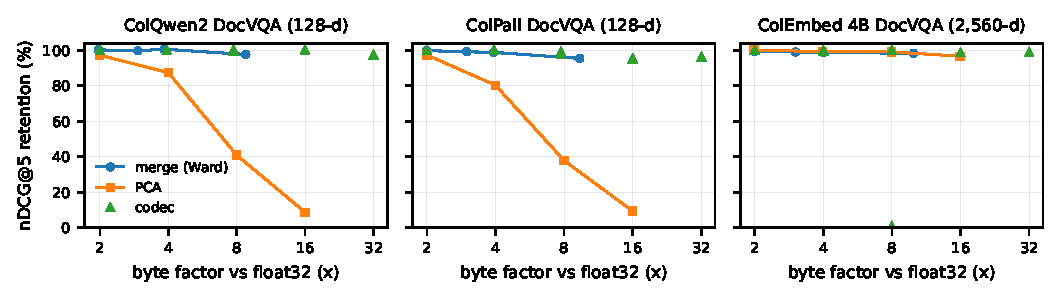
\includegraphics[width=\textwidth]{research_axes.pdf}
\caption{Retention against byte factor for each axis on DocVQA (measured). Vector merging
and per-vector codecs stay near float32 on all encoders. PCA collapses at 128 dimensions
but not at 2,560. Plain int4 collapses on ColEmbed~4B (the codec point near zero at
8$\times$, right panel).}
\label{fig:axes}
\end{figure*}

\textbf{Vector count drives search cost.} Exhaustive scan time fell to 0.52--0.53,
0.27--0.28 and 0.16 of float32 at 1/2, 1/4 and 1/8 of the vectors on all three 128-d
encoders. ColEmbed's within-device (GPU) ratios behave the same way. Halving or quartering
the width left 79--80\% and 74\% of the scan time. In the current implementation, codecs
made scans 1--7\% \emph{slower}, because codes are decoded to float32 before the product.
That is a property of the implementation, not of quantization (Section~\ref{sec:scale}).

\textbf{Merging is the quality-preserving vector reduction.} Merging to 1/4 of the
vectors cost at most 1.1 points on every 128-d dataset. A controlled attribution at
equal vector counts on six datasets isolated two effects. Ward clustering retains
$+0.7$ to $+3.7$ points more than K-means with plain means, and rescaling merged vectors
to their members' mean norm adds a further $+0.1$ to $+4.6$ points. All merging variants
beat random pruning in 51 of 54 comparisons, by up to 18 points at 1/20 of the vectors.

\textbf{Codecs.} Per-vector int8 and centred int4 stayed within about one point on every
encoder measured, including the text model (centred int4 98.6\%). Plain int4, 2-bit and
binary codes are model-dependent: plain int4 collapses on ColEmbed and loses 10 points on
the text model.

\textbf{Compression factors do not multiply, and the axes interact.} The actual byte
factor of a combination was 0.69--1.00 of the product of its single-axis factors at
128-d, because per-vector scales do not shrink with width. It was 0.53--1.00 on ColEmbed,
where the shared PCA basis also counts. Retention interactions were measured as
$I=R_{X+Y}-R_X R_Y$ with paired intervals:
\begin{itemize}
\item 14--34\% of two- and three-axis combinations showed a material interaction
($|I|\ge 0.01$, interval excluding 0);
\item every material interaction at 128-d was negative;
\item they concentrated in PCA combined with binary or centred int4, reaching $-18$
points, with the same direction in ColEmbed's point estimates;
\item merging combined with any codec was close to multiplicative.
\end{itemize}
The practical consequence is that axes must be evaluated jointly, not tuned as
independent knobs.

\textbf{Width changes the best storage pipeline.} On the in-sample storage frontier
(members with nDCG@5 retention $\ge 0.90$, all queries),
codecs alone cover the first $\approx$8$\times$ at 128-d. Merging plus a codec then
covers 8--125$\times$, and PCA enters only beyond $\approx$180$\times$. At 2,560-d,
projection plus a codec owns 8--63$\times$ (DocVQA) and up to 105$\times$ (InfoVQA). These
frontiers are in-sample. Held-out frontiers reproduced the axis composition within about
2 points, except at the extreme end.

%% ======================================================================
\section{Why Compression Differs Across Datasets}
\label{sec:datasets}

The shipped rule chose much less compression on DocVQA than on InfoVQA. At $T=0.95$ out
of sample it chose 11.8$\times$ against 72.7$\times$ (ColPali) and 32$\times$ against
355$\times$ (ColEmbed). Two explanations predict this: DocVQA representations could be
intrinsically more fragile under compression (\emph{compression sensitivity}), or
DocVQA's retention could simply be harder to \emph{certify} at a fixed query budget
(\emph{certification uncertainty}). The two are different quantities, and we measured
them separately.

\textbf{Intrinsic sensitivity is small.} For the same pipeline, pool retention on DocVQA
was within 0--2 points of InfoVQA. Only 0, 3 and 12 of 40 candidates
(ColQwen2, ColQwen2.5, ColPali) differed beyond their intervals.

\textbf{Certification uncertainty is large.} The certification standard error at
$n=225$, $\mathrm{sd}(c-Rb)/(\sqrt{225}\,\bar b)$, was 2.1--2.6$\times$ larger on DocVQA.
It splits about evenly into two parts: a lower mean baseline (the denominator) and a
larger per-query spread from near-boundary queries that both lose and gain under
compression.

\textbf{Relevance margins explain most of the gap} (Fig.~\ref{fig:q3}). Define a query's
relevance margin as the per-token score gap between its labelled page and the best other
page. 56--58\% of DocVQA queries fall in the two lowest margin quintiles, against
23--26\% of InfoVQA queries. Two observational analyses close most of the
certification-SE gap:
\begin{itemize}
\item reweighting InfoVQA to DocVQA's margin distribution closes 61--81\%;
\item restricting DocVQA to its positive-margin half closes 84--120\%. That half is a
ceiling subset in which baseline nDCG@5 is $\approx$1, so it overstates the match.
\end{itemize}
These analyses are observational, not causal. A residual remains, larger for ColPali.
We therefore conclude that \emph{DocVQA receives less certified compression primarily
because its quality is harder to certify, not because its representations are
intrinsically less compressible}, with residual uncertainty.

\begin{figure}[t]
\centering
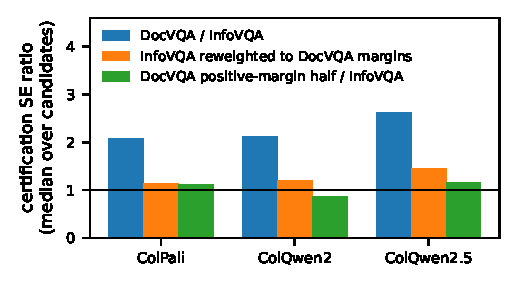
\includegraphics[width=\columnwidth]{research_q3.pdf}
\caption{Ratio of the $n=225$ certification standard error between DocVQA and InfoVQA
(median over 40 candidates; measured). Matching InfoVQA to DocVQA's relevance-margin
distribution, or restricting DocVQA to its positive-margin half, removes most of the
gap. The analyses are observational, not causal.}
\label{fig:q3}
\end{figure}

%% ======================================================================
\section{Quality-Constrained Selection and Certification}
\label{sec:cert}

\textbf{The shipped rule is empirically safe but not certified.} Across 20 random
calibration/held-out splits per cell, the shipped 0.999-bound rule met its target on the
held-out half in 355 of 360 choices for the 128-d encoders and SciFact, and in 119 of 120
for ColEmbed. The worst miss was 97.4\% against 0.99. Choosing by the point estimate met
the target in only 10--100\% of splits per cell. Because the splits reuse one query pool
per corpus, these counts are empirical summaries, not rates with population-level
guarantees.
\begin{itemize}
\item \emph{Looser targets always buy at least as much compression}
(Fig.~\ref{fig:targets}): in every dataset--encoder cell, the median chosen compression
never decreased as the target loosened.
\item \emph{The rule has no post-selection statement}: in population resampling it
missed the finite-pool target in up to 26\% of draws at $n=50$.
\end{itemize}

\begin{figure}[t]
\centering
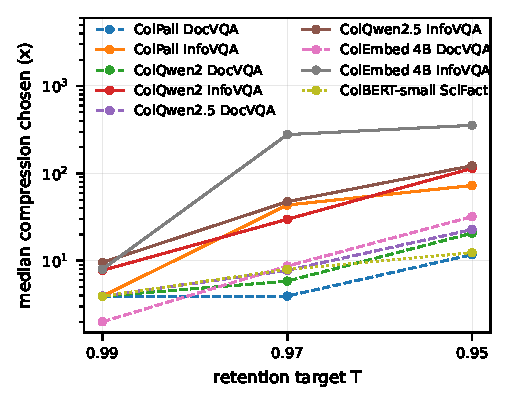
\includegraphics[width=\columnwidth]{research_targets.pdf}
\caption{Median compression chosen out of sample by the shipped rule at three retention
targets (20 splits per cell; measured). Compression is dataset-dependent and never
decreases as the target loosens. These are empirical results without a post-selection
guarantee.}
\label{fig:targets}
\end{figure}

\textbf{A certified alternative (Method C).} We apply two established ideas. Exact
p-values for the bounded mean in (\ref{eq:boundedmean}) come from testing by
betting~\cite{waudbysmith2024betting}, with Ville's inequality~\cite{ville1939}. Each
candidate family is walked in its pre-specified compression order by fixed-sequence
testing~\cite{westfall2001fixedsequence}, in the style of learn-then-test risk
control~\cite{angelopoulos2021ltt}, at level $\delta/F$ for $F$ families. The smallest
rejected configuration is deployed. Under i.i.d.\ queries, a fixed corpus and stages
fitted without calibration queries, this gives
\begin{equation}
\Pr\bigl(\text{deploy} \wedge R_Q(\hat k) < T\bigr) \le \delta
\end{equation}
for the \emph{selected} configuration $\hat k$.

Method C is a validated application of known methods, providing a conditional,
finite-sample guarantee. It is not a new statistical method, it is not a guarantee for
the shipped rule, and it does not hold for other corpora, growing corpora, or query
distributions unlike the calibration pool.

\textbf{Validation.} In population resampling on ColPali and ColQwen2, and in a
held-back confirmation frozen before loading ColQwen2.5 and SciFact, the bound held in
every check:
\begin{itemize}
\item 27 of 27 held-back cells, with a maximum observed miss of 0.05\% at $\delta=0.05$;
\item with $\le 225$ calibration queries, C deployed at $T=0.95$ on all three held-back
datasets (ColQwen2.5 DocVQA 7.8$\times$, ColQwen2.5 InfoVQA 76.0$\times$, SciFact
11.8$\times$), and at $T=0.97$ only on InfoVQA;
\item it was never run on ColEmbed, for lack of per-query data.
\end{itemize}

\textbf{The 0.99 limit.} Consider any test valid at level $\delta$, and contaminate a
lossless candidate with an $\varepsilon$ mass of total failures so that its retention
equals $T$. Rejecting the null with probability at least $1/2$ then requires
$n\ge \log(1/(2\delta))/(-\log(1-\varepsilon))$, where
$\varepsilon=\beta(1-T)/(T+\beta(1-T))$ and $\beta$ is the mean baseline score. At
$T=0.99$ and $\delta=0.05$ this needs 250--392 queries on our pools, more after the
$\delta/F$ correction. \emph{No distribution-free method can certify $T=0.99$ with 225
or fewer calibration queries here}, which is why a 0.95 result does not transfer to
0.99.

%% ======================================================================
\section{Search Cost, Memory and Scaling}
\label{sec:scale}

\textbf{Measured scaling.} We tiled the ColQwen2 DocVQA corpus 1, 2, 4 and 8 times
(500--4,000 identical duplicated pages, used for timing only) and timed exhaustive scans
(Fig.~\ref{fig:scan}). All six configurations were linear in stored vectors: the time at
4,000 pages was 0.98--1.08 of eight times the 500-page time, with $R^2\ge 0.999$. The
per-vector cost was similar across codecs (37--39\ms\ per million vectors per query) and
only about 22\% lower after halving the width. Vector count therefore remains the
latency lever.

\begin{figure}[t]
\centering
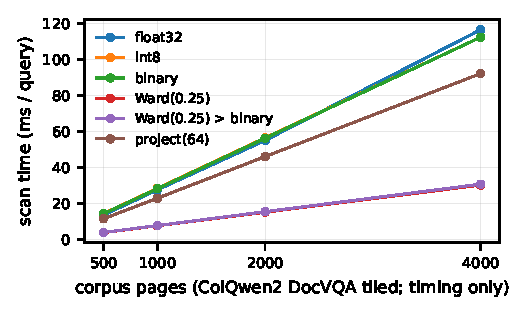
\includegraphics[width=\columnwidth]{research_scan.pdf}
\caption{Exhaustive scan time against corpus size on tiled ColQwen2 DocVQA (duplicated
pages; timing only, no retrieval metric; measured on one laptop CPU). Time is linear in
stored vectors over 500--4,000 pages.}
\label{fig:scan}
\end{figure}

\textbf{Two-tier search.} Rescoring 50 candidates per query with the previous per-query
loop cost $\approx$11.2\ms\ per query, flat in corpus size. The batched implementation
cost 1.53--4.03\ms\ as the number of distinct candidate pages grew from 500 to 3,984.
Its advantage therefore fell from 7.4$\times$ to 2.8$\times$ as overlap between queries
fell; below that overlap it is untested. Extrapolating linearly (projected), the
exhaustive hot stage exceeds the rescoring cost beyond $\approx$1,300 pages. Two-tier
indexing thus reduces RAM by about 30$\times$ relative to int8 but does not change the
linear scaling class.

\textbf{Native compressed-code scoring.} Scoring int8 codes directly with an available
mixed-precision kernel, or binary codes with lookup tables, reproduced the current
rankings up to float32 near-ties. It was 24--34$\times$ and 28--30$\times$ slower than
decode-then-BLAS. This is a negative result \emph{on this tested software stack} (numpy
and PyTorch on one CPU, with no compiled kernels), not a general property of compressed
retrieval.

\textbf{Projected resources} (arithmetic on measured per-page bytes). Storage and RAM
scale linearly in pages plus a small fixed shared state. At 1M pages, ColQwen2 projects
to 383\,GB in float32, 12\,GB as binary codes and 3.1\,GB merged to 1/4 then binarized.
Under an 8\,GB RAM budget, uncompressed 128-d indexes fit 16--23k pages, and merged
binary fits 2.0--2.8M. These are projected resource figures, not demonstrated
capability. Exhaustive search at that scale projects to several seconds per query on our
laptop, and retrieval quality beyond 500 pages was not measured.

%% ======================================================================
\section{Generalization Across Models and Corpora}
\label{sec:general}

Table~\ref{tab:general} classifies the findings against the tested set. Our overall
verdict is \emph{supported with scope limitations}.

\begin{table}[t]
\centering
\caption{Generalization within the tested set (four visual encoders across two widths,
one text encoder, three corpora). ``Replicated'' means observed on every encoder and
corpus where it was measured.}
\label{tab:general}
\setlength{\tabcolsep}{3pt}
\begin{tabular}{p{0.62\columnwidth}p{0.30\columnwidth}}
\toprule
finding & status \\
\midrule
vector count drives exhaustive search cost & replicated \\
relative merging beats pruning, preserves quality to $\approx$1/4 & replicated \\
int8 per vector near-lossless & replicated \\
centred int4 near-lossless ($\le$1.4 points) & replicated \\
factors do not multiply; PCA + coarse codecs antagonistic & replicated (ColEmbed: points only) \\
two-tier keeps quality, cuts RAM & replicated \\
certification difficulty drives dataset differences & replicated (DocVQA vs InfoVQA) \\
Method C's conditional validity & replicated (4 encoders, 3 corpora; not ColEmbed) \\
\midrule
dimension reduction & model-specific \\
plain int4; centred binary; 2-bit/binary strength & model-specific \\
absolute merge thresholds & do not transfer \\
amount of certifiable compression & dataset-specific \\
codec speed (decode-first) & implementation-specific \\
\bottomrule
\end{tabular}
\end{table}

Model dependence is concrete:
\begin{itemize}
\item PCA to $d/4$ loses 9--20 points at 128 dimensions but at most 0.9 points at
$d/8$ for ColEmbed;
\item plain int4 ranges from lossless (ColQwen) to collapse (ColEmbed);
\item centred binary collapses on the text model, whose vectors occupy a narrow cone;
\item a fixed merge radius merges about half as much on ColQwen as on ColPali.
\end{itemize}
Relative per-page budgets transferred where absolute thresholds did not. SciFact
confounds the text model with a text corpus, so no claim about text corpora in general
is supported.

%% ======================================================================
\section{Comparison With Prior Work}
\label{sec:prior}

\textbf{Related methods.}
\begin{itemize}
\item \emph{Token reduction}: Ward token pooling is prior work~\cite{clavie2024pooling},
and OptiVision's merge stage implements it. Merging also outperforms pruning in
Light-ColPali~\cite{lightcolpali} and in a recent comparison of training-free methods
on text~\cite{jha2026comparison}. Adaptive pruning and prune-then-merge methods target
ColPali-family models~\cite{docpruner2025,sculpting2026,adamerge2026}.
\item \emph{Codes and engines}: residual compression and engines such as
ColBERTv2/PLAID and EMVB~\cite{colbertv2,plaid,emvb} and fixed-dimensional encodings
(MUVERA~\cite{muvera}) are established. So are binary multi-vector codes with float
rescoring and shortlist-and-rescore designs~\cite{vespa2024colpali,qdrant}.
\item \emph{Statistics}: our selection procedure uses known statistical
tools~\cite{waudbysmith2024betting,westfall2001fixedsequence,angelopoulos2021ltt}.
\end{itemize}

\textbf{The one directly comparable setup.} Our survey found a single published setup
with the same checkpoints (ColPali~v1.3 and ColQwen2~v1.0) and the same ViDoRe~V1
subsets: Structural Anchor Pruning (SAP)~\cite{structuralanchor2026}.
\begin{itemize}
\item \emph{The disagreement}: at about 1/10 of the vectors, our measured Ward merging
retains 4--10 points more than SAP's reported K-means baseline.
\item \emph{Mechanism choices explain part of it}: a controlled attribution on our data
found that clustering and rescaling choices account for part of the gap.
\item \emph{Evaluation is not the cause}: aligning our evaluation with the official
ViDoRe legacy and MTEB pipelines changed results by at most 0.65 points.
\item \emph{What remains}: on ColPali, random-pruning controls agree with SAP within 1.6
points. On ColQwen2 they disagree by up to 14 points before any compression method is
applied, which points to an upstream difference (plausibly encoding settings).
\end{itemize}
The discrepancy is unresolved. We report it as an unresolved disagreement, \emph{not}
as evidence that either approach is better or worse.

%% ======================================================================
\section{Limitations and Open Questions}
\label{sec:limits}

\textbf{Scope.}
\begin{itemize}
\item Four visual encoders across two widths (three of them 128-d), one text encoder,
and three corpora. The visual corpora are 500-page ViDoRe~V1 subsets.
\item One query pool per corpus, so split-based rates are summaries, not population
estimates.
\item ColEmbed: aggregate results only, with GPU timing.
\item Not covered: 4,096-dimensional or other model families; ViDoRe~V2/V3; retrieval
quality beyond 500 pages (an audit found lossy configurations losing 0--3 points from
100 to 500 pages); timing beyond 4,000 duplicated pages.
\end{itemize}

\textbf{Implementation and statistics.}
\begin{itemize}
\item Timing comes from one laptop with two CPU power states.
\item Codec-speed and native-kernel results are specific to this implementation.
\item The library does not yet persist centred int4 or 2-bit codecs, or the PCA basis.
\item Method C assumes i.i.d.\ queries and a fixed corpus; the shipped rule's success
rates are empirical.
\item Our literature survey covered multi-vector compression and retrieval engines, not
the statistical-selection literature.
\end{itemize}

\textbf{Open questions.}
\begin{itemize}
\item the ColQwen2 discrepancy with SAP;
\item the residual DocVQA certification gap;
\item the cause of plain int4's collapse at 2,560 dimensions;
\item batched rescoring at very low candidate overlap;
\item retrieval quality at large corpus sizes;
\item whether compiled native kernels outperform decode-then-BLAS;
\item sublinear candidate generation, which would be needed to change the scaling class.
\end{itemize}

%% ======================================================================
\section{Discussion}
\label{sec:discussion}

Three lessons follow from the evidence, each within its tested scope:
\begin{itemize}
\item \emph{Compression cost and certification cost are distinct}, and on DocVQA the
second dominates. Reporting retention without the uncertainty of its estimate can make
a dataset look less compressible than it is.
\item \emph{Axes are not independent knobs.} Byte factors do not multiply, and some
pairings, notably projection followed by coarse codes, lose more than their parts.
\item \emph{A smaller index is not a faster search in a decode-first implementation.}
Only fewer vectors reduced exhaustive cost here.
\end{itemize}
Each lesson is an empirical finding established on our tested set. Whether any is new
relative to the complete literature is not established by this work.

%% ======================================================================
\section{Reproducibility}
\label{sec:repro}

Every quantitative claim comes from frozen, pre-registered studies on the
\texttt{research-investigation} branch of the OptiVision repository. The summary is in
\texttt{reports/research/PAPER\_SUMMARY.md}, with per-study reports:
\begin{itemize}
\item Q3: dataset differences;
\item Q4: compression axes;
\item Q5/Q6: native scoring;
\item Q7, E7a, E7c: prior-work comparison;
\item Q8: scaling;
\item Q9: generalization;
\item Q10: contribution classification;
\item \texttt{reports/engineering/batched\_rescore}: batched rescoring.
\end{itemize}
The figures are regenerated from those reports by \texttt{paper/make\_figs\_research.py}.
Encoded vectors are not stored in the repository; per-query result stores and scripts
are.

%% ======================================================================
\section{Conclusion}

OptiVision is a model-agnostic engineering framework for quality-constrained
multi-vector compression. A systematic, pre-registered evaluation across four visual
encoders, one text encoder and three corpora establishes several cross-model empirical
findings:
\begin{itemize}
\item stored vector count governs exhaustive search cost;
\item relative merging and per-vector int8 and centred int4 preserve quality;
\item compression factors do not multiply, and the axes interact;
\item dataset differences in certified compression stem mainly from certification
difficulty.
\end{itemize}
It also identifies clear model-, dataset- and implementation-dependent boundaries:
dimension reduction, low-bit codecs, the amount of certifiable compression, and codec
speed. A known post-selection procedure gives a conditional finite-sample statement for
the selected configuration, with a hard query-count limit at high targets. These
findings are established within the tested scope; their novelty relative to the full
literature is not.

%% ======================================================================
\begin{thebibliography}{00}

\bibitem{colbert}
O. Khattab and M. Zaharia, ``ColBERT: Efficient and Effective Passage Search via
Contextualized Late Interaction over BERT,'' in \emph{Proc. 43rd Int. ACM SIGIR
Conf. on Research and Development in Information Retrieval}, 2020, pp. 39--48.

\bibitem{colbertv2}
K. Santhanam, O. Khattab, J. Saad-Falcon, C. Potts and M. Zaharia, ``ColBERTv2:
Effective and Efficient Retrieval via Lightweight Late Interaction,'' in
\emph{Proc. NAACL-HLT}, 2022, pp. 3715--3734.

\bibitem{colpali}
M. Faysse, H. Sibille, T. Wu, B. Omrani, G. Viaud, C. Hudelot and P. Colombo,
``ColPali: Efficient Document Retrieval with Vision Language Models,''
in \emph{Proc. Int. Conf. on Learning Representations (ICLR)}, 2025.

\bibitem{colembed}
NVIDIA, ``nemotron-colembed-vl-4b-v2,'' model card, Hugging Face, revision
0ed152d9. [Online]. Available:
\url{https://huggingface.co/nvidia/nemotron-colembed-vl-4b-v2}

\bibitem{beir}
N. Thakur, N. Reimers, A. R\"uckl\'e, A. Srivastava and I. Gurevych, ``BEIR: A
Heterogeneous Benchmark for Zero-shot Evaluation of Information Retrieval Models,''
in \emph{Proc. NeurIPS Datasets and Benchmarks Track}, 2021.

\bibitem{mteb}
N. Muennighoff, N. Tazi, L. Magne and N. Reimers, ``MTEB: Massive Text Embedding
Benchmark,'' in \emph{Proc. EACL}, 2023.

\bibitem{ward1963}
J. H. Ward, ``Hierarchical Grouping to Optimize an Objective Function,''
\emph{J. Amer. Statist. Assoc.}, vol. 58, no. 301, pp. 236--244, 1963.

\bibitem{clavie2024pooling}
B. Clavi\'e, A. Chaffin and G. Adams, ``Reducing the Footprint of Multi-Vector
Retrieval with Minimal Performance Impact via Token Pooling,'' in \emph{Findings
of the Association for Computational Linguistics: EMNLP 2024}, 2024.
arXiv:2409.14683.

\bibitem{lightcolpali}
Y. Ma, J. Li, Y. Zang, X. Wu, X. Dong, P. Zhang, Y. Cao, H. Duan, J. Wang,
Y. Cao and A. Sun, ``Towards Storage-Efficient Visual Document Retrieval: An
Empirical Study on Reducing Patch-Level Embeddings,'' in \emph{Findings of the
Association for Computational Linguistics: ACL 2025}, 2025. arXiv:2506.04997.

\bibitem{jha2026comparison}
R. Jha, C. Zuo, R. Kriz and B. Van Durme, ``A Brief Comparison of Training-Free
Multi-Vector Sequence Compression Methods,'' \emph{arXiv preprint
arXiv:2603.22434}, 2026.

\bibitem{docpruner2025}
Y. Yan, G. Xu, X. Zou, S. Liu, J. Kwok and X. Hu, ``DocPruner: A
Storage-Efficient Framework for Multi-Vector Visual Document Retrieval via
Adaptive Patch-Level Embedding Pruning,'' \emph{arXiv preprint
arXiv:2509.23883}, 2025.

\bibitem{sculpting2026}
Y. Yan, M. Ou, Y. Cao, X. Zou, J. Huo, S. Liu, J. Kwok and X. Hu, ``Sculpting
the Vector Space: Towards Efficient Multi-Vector Visual Document Retrieval via
Prune-then-Merge Framework,'' in \emph{Findings of the Association for
Computational Linguistics: ACL 2026}, 2026. arXiv:2602.19549.

\bibitem{adamerge2026}
J. You and K. Ni, ``AdaMerge: Tuning-Free Patch Compression for Multi-Vector Visual
Document Retrieval,'' \emph{arXiv preprint arXiv:2609.22562}, 2026.

\bibitem{structuralanchor2026}
Z. Liu, Z. Hu, Y. Zhang and Y. Xiao, ``Structural Anchor Pruning:
Training-Free Multi-Vector Compression for Visual Document Retrieval,''
\emph{arXiv preprint arXiv:2601.20107}, v3, 2026.

\bibitem{plaid}
K. Santhanam, O. Khattab, C. Potts and M. Zaharia, ``PLAID: An Efficient Engine for
Late Interaction Retrieval,'' in \emph{Proc. 31st ACM Int. Conf. on Information and
Knowledge Management (CIKM)}, 2022.

\bibitem{emvb}
F. M. Nardini, C. Rulli and R. Venturini, ``Efficient Multi-vector Dense Retrieval
with Bit Vectors,'' in \emph{Proc. European Conf. on Information Retrieval (ECIR)},
2024.

\bibitem{muvera}
L. Dhulipala, M. Hadian, R. Jayaram, J. Lee and V. Mirrokni, ``MUVERA: Multi-Vector
Retrieval via Fixed Dimensional Encodings,'' in \emph{Advances in Neural Information
Processing Systems (NeurIPS)}, 2024.

\bibitem{vespa2024colpali}
J. K. Bergum, ``Scaling ColPali to Billions of PDFs with Vespa,'' Vespa blog,
Sep. 2024. [Online]. Available: \url{https://blog.vespa.ai/scaling-colpali-to-billions/}

\bibitem{qdrant}
Qdrant, ``Multivectors, Binary Quantization and Rescoring,'' Qdrant
Documentation. [Online]. Available: \url{https://qdrant.tech/documentation/}

\bibitem{waudbysmith2024betting}
I. Waudby-Smith and A. Ramdas, ``Estimating Means of Bounded Random Variables by
Betting,'' \emph{J. Roy. Statist. Soc. Ser. B}, vol. 86, no. 1, pp. 1--27, 2024.

\bibitem{ville1939}
J. Ville, \emph{\'Etude critique de la notion de collectif}. Paris:
Gauthier-Villars, 1939.

\bibitem{westfall2001fixedsequence}
P. H. Westfall and A. Krishen, ``Optimally Weighted, Fixed Sequence and Gatekeeper
Multiple Testing Procedures,'' \emph{J. Statist. Plann. Inference}, vol. 99, no. 1,
pp. 25--40, 2001.

\bibitem{angelopoulos2021ltt}
A. N. Angelopoulos, S. Bates, E. J. Cand\`es, M. I. Jordan and L. Lei, ``Learn then
Test: Calibrating Predictive Algorithms to Achieve Risk Control,'' \emph{arXiv
preprint arXiv:2110.01052}, 2021.

\end{thebibliography}

\end{document}
